\chapter{Introduction\label{chap:introduction}}
\section{Motivation}
% Drug discovery is important. 
Drug discovery is the process of identifying new medicines and bringing them to
market. The discovery of novel pharmaceutical treatments has been a major driver
of quality of life over the centuries. While discovery of new drugs has started 
in serendipitous and lucky discoveries, advances in science and technology  
led to an ever more systematic and data-driven approach, especially over the
last decades. 

% Traditional way of finding candidates.
One of the key challenges of the drug discovery process is the identification
of novel promising drug candidates. The efficacy of a drug is usually determined by its ability
to interact with a biological target in the body. To find such molecules,
the traditional approach is to synthesize and test the molecules efficacy first in laboratory
experiments, and finally in clinical studies. However, this process is usually very expensive, time-consuming
and can involve risks for patients.

% Computer aided drug discovery
Computer aided drug discovery (CADD) aims to accelerate the drug discovery
process using computational methods. Applications range from basic chemical
information processing, over physical simulation of molecular interactions, to
sophisticated machine learning methods. Advances in deep learning
have led to breakthroughs in many different
areas of drug discovery \citep{chenRiseDeepLearning2018}, including highly accurate protein structure prediction 
achieved by AlphaFold \citep{todo}, chemical property prediction
\citep{mayrDeepToxToxicityPrediction2016,todo}, synthesis planning
\citep{seglerNeuralSymbolicMachineLearning2017} and molecule generation
\citep{todo}. These advances help by reducing the need for expensive 
wet-lab experiments and can assist chemists in drug design tasks. 

% Significance and objectives of the thesis
In this thesis we focus on generative models for molecules. Generative models
are a class of machine learning models that generate molecular structures
relevant to a given task. However, the evaluation of generative models is
challenging, as the outputs of these models are usually complex, structured
objects, and there are often no straightforward ways to evaluate the quality or
relevance of the generated molecules. In this thesis, we address this issue by
proposing new evaluation metrics and benchmarks for generative models.

% Synthesis planning
We also study the application of generative models to computer-aided synthesis
planning (CASP). CASP tools assist chemists in the task of synthesizing target
molecules. These tools rely on retrosynthesis prediction models, which predict
the reactants that can be used to synthesize a target molecule. We propose a
novel retrosynthesis prediction model that improves the generalization capabilities 
of template-based models. We also propose new evaluation metrics and highlight
trade-offs between accuracy and throughput in retrosynthesis prediction.

% PROMISE
This thesis is structured as follows. In \cref{sec:drug-design} we give an
overview of small molecule drug design, the drug discovery pipeline 
and how computer aided drug discovery can help to accelerate this process.
In \cref{sec:generative-models} we give an overview of generative models for
molecules and discuss the challenges of evaluating these models In \cref{sec:retrosynthesis} 
we give a short overview of computer-aided synthesis planning.
\Cref{sec:retrosynthesis} gives an overview of retrosynthesis prediction and
the associated challenges. \Cref{sec:aims-objectives} gives an overview of the
aims and objectives of this thesis. \Cref{sec:publications} lists the publications 
that are part of this thesis and related publications. 
\Cref{chap:publications} reprints the publications and
their corresponding supplementary material. Finally, \Cref{chap:conclusion}
concludes the thesis and gives an outlook on future work.



% \begin{minipage}
% : Rational drug discovery.
% This approach starts with the identification of a biological target in the body 
% which is hypothesized to be associated with a disease phenotype. 
% One then attempts to find a small molecule that can change the activity of 
% the target in the desired way. While this way of searching for new drugs 
% is more direct than phenotypic drug discovery the identification of 
% drug targets can be challenging and given the complex interconnectedness 
% of biochemical pathways, it is not fully understood how some drugs work, 
% which goes even for highly popular ones.

% Phenotypic drug discovery takes this trial-and-error approach and applies it 
% in a systematic manner. The focus in this approach, which is also called forward 
% pharmacology, lies on screening collections of small molecules or other potential 
% medicines for pharmaceutical effects. Once a pharmacologically active molecule 
% has been found the aim is to discover how to use it's effect therapeutically. 
% This process can proceed without knowing the biochemical mode of action, of how 
% a drug actually achieves its effect. 

% How were new medicines discovered?
% David C. Swinney & Jason Anthony 
% Lots of molecules also by phenotypic screening

% One of core goals in both approaches is to find molecules with a desired
% pharmacological profile, which includes primarily the ability of a molecule to
% modify a target, but also other important
% properties, e.g. absorption, distribution, metabolism, excretion or toxicity. 
% To find such molecules, specially designed wet-lab experiments called \emph{assays} 
% are usually use to measure these properties of interest. The number of tested 
% molecules can range from numbers in the tens to millions of tested molecules
% in high-througput screening. 

% \emph{Computer-aided drug design} aims to reduce the need 
% for these expensive experiments using computational methods. 
% The field of quantitative structure activity/property relationship (QSAR/QSPR)
% aims to find an accurate computational model of the drug-target interaction. 
% Structure-based methods make use of the known structures of the drug and target 
% and calculate binding affinity using physical modelling. 
% In contrast, ligand-based methods find links between molecular structures
% and measured experimental outcomes. In recent years, machine learning methods 
% have shown great promise at modelling these relationships. 
% Using these models one can prioritize which of the molecules available in a screening 
% collection to test next, to avoid wasting ressources on unpromising compounds.

% However, this approach of virtual screening is limited to existing screening collections
% and computational constraints. The $~10^{12}$ \citep{todo} molecules that can be realistically 
% evaluated fall far short of the $10^{23}$-$10^{60}$ drug-like molecules 
% which are estimated to exist \citep{todo}, and necessarily miss out on promising drug candidates.
% Generative models aim to alleviate this problem, by using the QSAR/QSPR function as a guiding signal 
% in order to be able to explore chemical space in a goal-directed manner. 
% The evaluation 

% However, the process of bringing a new drug to market is a long, expensive, and risky endeavor.
% Estimates of bringing a new drug to market range between 2.6 and xxx 
% billion USD \citep{todo}. When successful, however, a new drug can be a major source of
% relief for patients.

% % Traditional way of finding candidates.
% One of the key challenges of the drug discovery process is the identification
% of novel promising drug candidates. Traditionally, this is done by synthesizing
% and testing the molecules efficacy in a laboratory and clinical studies. 
% However, this process is usually very expensive, time-consuming and can be risky for 
% patients. 

% % ML can help to find promising candidates
% Machine learning (ML) and deep learning (DL) have the potential to accelerate
% the drug discovery process. Recent advances in ML, especially in the subfield of deep learning
% have led to a surge in interest in applying ML and DL to drug discovery, 
% culminating in breakthroughs such as AlphaFold \citep{todo}. 
% In this thesis, we focus on two key areas where ML and DL can help to accelerate
% the drug discovery process: generative models for molecules and computer-aided
% synthesis planning (CASP).
% \end{minipage}

\section{Small molecule drug design\label{sec:drug-design}}
\subsection{Requirements for small molecule drugs}
Small molecule drugs are the major kind of medicines in use, with as much as
90\% of global sales \citep{makurvetBiologicsVsSmall2021}.
For a small molecule to be a viable drug candidate it needs to fulfill a whole range 
of properties \citep{todo}:
\begin{itemize}
    \item \textbf{On-target activity:} The molecule needs to be active against
    the desired target in order for it to show the desired therapeutic effect.
    On a molecular level this means that the molecule needs to bind to the target
    and modulate its activity in the desired way. 
    \item \textbf{Pharmacokinetics:} The molecule must have favourable
    pharmacokinetic properties such as adsorption, distribution, metabolism and
    excretion (ADME). ADME determine how the molecule is absorbed into the
    body, how it is distributed in the body, how it is metabolized and how it is
    excreted from the body. These properties are crucial for the molecule to
    reach the target in the body and to be metabolized in a safe manner and to 
    finally be excreted from the body.
    \item \textbf{Toxicity:}  The absence of toxic effects is crucial, as the
    molecule must be well-tolerated and devoid of any potential harmful side
    effects. Toxicity can be caused by a range of factors, including off-target
    interactions, metabolic byproducts or allergies.
    \item \textbf{Specificity:}  The molecule should exhibit high specificity,
    selectively interacting with the intended target while minimizing
    undesirable off-target interactions. Off-target binding can lead to adverse
    side effects and potentially compromise the drug's safety and efficacy
    profile.
    \item \textbf{Synthesis:} The molecule must be synthesizable in a
    cost-effective manner to be practically useful.
    \item \textbf{Patentability:} The molecule must be novel and not infringe on
    any existing patents. While in general this is not needed for a drug to work, 
    this constitutes a significant issue in practice.
\end{itemize}

\subsection{The drug discovery pipeline}
The process of discovering a new drug is a complex and multi-faceted task. The
cost of bringing a new drug to market is estimated to be between 2.6 and 3.0
billion USD \citep{todo} and the process can take up to 10-15 years
\citep{todo}. The chances of success are low, with only about 10\% of drugs that
enter clinical trials eventually being approved by regulatory agencies
More specifically, the success rates
in Phase I/II/III and the final regulatory approval are 63\%, 31\%, 58\% and
85\% respectively \citep{mullardParsingClinicalSuccess2016}. This translates to
63\%, 19.5\%, 11.3\% and 9.6\% of projects that make it to the respective stages
\citep{mullardParsingClinicalSuccess2016}.

The drug discovery pipeline is usually divided into multiple stages, depicted in
\Cref{fig:drug-discovery-pipeline}. The stages are as follows:
\begin{figure}
    \centering
    \includegraphics[width=\textwidth]{figures/drug-discovery-pipeline.pdf}
    \caption{The drug discovery pipeline starts with the identification of a
    biological target. Once a target is identified, readily available molecules
    are screened for their activity against the target in high-throughput
    screening. Promising hits are then modified and optimized to lead compounds.
    These lead compounds are then further optimized and tested in preclinical.
    Finally, the most promising candidates are tested in clinical trials and
    eventually approved by regulatory agencies. The stages in the blue box are
    highly amenable to machine learning and computational methods and are the
    focus of this thesis. \label{fig:drug-discovery-pipeline}}
\end{figure}
\begin{itemize}
    \item \textbf{Target identification:} The first stage is target identification, 
    where a biological target is identified that is hypothesized to be associated
    with a disease phenotype.
    \item \textbf{Hit discovery:} In the hit discovery stage molecules are
    screened for their activity against the target in high-throughput screening (HTS).
    These lab experiments ,often referred to as assays, are used to measure the
    activity of the molecules against the target in vitro. HTS is resource
    intensive and time-consuming.
    \item \textbf{Hit-to-lead:} Promising hits are then modified and optimized
    to lead compounds. In this stage, the optimization is primarily focused on
    improving the activity of the molecule against the target. This is usually 
    done in a DMTA (Design-Make-Test-Analyze) cycle, where the molecule is
    designed, synthesized, tested in vitro. The results are then analyzed and the cycle 
    continues until a satisfactory lead compound is found.
    \item \textbf{Lead optimization:} The lead compounds are then further
    optimized to improve their properties, such as pharmacokinetics, toxicity or
    specificity. This is usually done in a DMTA cycle as in the
    hit-to-lead stage and also involves the synthesis and testing of the
    molecules in vitro.
    \item \textbf{Preclinical development:} The most promising candidates are then tested in
    preclinical studies. These studies are usually done in animals and are used
    to assess the safety and efficacy of the drug candidate in vivo. 
    \item \textbf{Clinical trials:} Finally, the candidates that pass the
    preclinical studies are tested in humans in clinical trials. 
    These are usually divided into three phases, where the safety and efficacy
    of the drug are tested in increasing numbers of patients. 
    Phase I trials are mainly focused on the safety of the drug, Phase II trials
    are focused on the efficacy of the drug and Phase III trials are focused on
    the safety and efficacy of the drug in a larger population.
    \item \textbf{Regulatory approval:} The final stage is the regulatory
    approval, where the drug is approved by regulatory agencies such as the FDA
    in the US or the EMA in Europe. 
\end{itemize}

The hit discovery, hit-to-lead and lead optimization (blue box in
\Cref{fig:drug-discovery-pipeline}) are highly amenable to machine learning and
computational methods and are the focus of this thesis. Specifically 
we will focus on generative models for molecules, which can help to 
find hits in the hit discovery stage and optimize lead compounds in the
hit-to-lead and lead optimization stages. Furthermore we will look at 
computer-aided synthesis planning (CASP) tools, which can help to find
synthesis routes for promising molecules in the hit discovery, hit-to-lead and lead optimization
stages.

\subsection{Efficiently navigating chemical space}
% Drug discovery equals searching chemical space 
The drug discovery pipeline can be seen as a structured process of searching
chemical space for molecules that can successfully be used as medicines.
As a trial and error process, this search needs to be conducted in a 
systematic manner. The design-make-test-analyze (DMTA) cycle is a
common approach to proceed throughout the drug discovery pipeline.
The steps in this cycle are as follows:
\begin{itemize}
    \item \textbf{Design:} The first step is the design of the molecule to be
    tested. This can be done using a variety of methods, ranging from 
    intuition and experience of medicinal chemists to computational methods.
    \item \textbf{Make:} The designed molecules are synthesized and purified in
    the laboratory. This step is usually done by chemists and can be a complex
    and time-consuming process.
    \item \textbf{Test:} The synthesized molecule is then tested in vitro or in
    vivo to measure its activity against the target and its pharmacokinetic
    properties.
    \item \textbf{Analyze:} The results of the test are then analyzed to
    determine whether the experiment was successful and to guide the next
    iteration of the DMTA cycle.
\end{itemize}

\subsection{Computer-Aided Drug Discovery}
Computer-aided drug discovery (CADD) aims to accelerate the drug discovery
process using computational methods, offering support throughout all stages of 
the drug discovery pipeline and all steps of the DMTA cycle.

Virtual screening (VS) constitutes a key application of CADD. VS methods aim to
predict molecular properties of interest, such as the activity of a molecule
against a target, its pharmacokinetic properties or its toxicity. These
predictions can be used to prioritize which molecules to test next, to avoid
wasting resources on unpromising compounds. Therefore it helps in the design
step of the DMTA cycle, by helping to design the next batch of experiments. 
Structure-based methods constitute one of the most popular approaches to VS. These methods use the known
structure of the target to predict the activity of a molecule against the target.
This approach has been boosted by advances in protein structure prediction, such
as AlphaFold \citep{todo}. Ligand-based methods are another popular approach to
VS. These methods find links between molecular structures and measured
experimental outcomes. In recent years, machine learning methods have shown
great promise in modeling these relationships. 

However, these discriminative methods have limitations and fail to help in the
other steps of the DMTA cycle. Generative models offer complementary methods
which can help in the analyze, design and make steps of the DMTA cycle. Key
applications of generative models in drug discovery are the generation of
molecules with desired properites, the optimization of lead compounds and the
prediction of chemical reactions to help synthesize molecules. While VS methods
can be seen as an in silico replacement for experiments, generative models for
molecules function more like a virtual chemist, designing and optimizing
molecules and through modelling chemical reactions.

In recent years, there has been a resurgence of interest in generative models,
triggered by advances in deep learning. These models represent a significant
shift in how we approach drug discovery, providing new methods to innovate and
optimize the process. In the following section, we will give a more detailled 
overview of generative models for molecules and their applications in drug discovery.

% \begin{itemize}
%     \item \textbf{Proxy models:} One way is to use proxies, which 
%     aim at approximating the outcome of an expensive experiment at a lower cost.
%     Conducting a clinical trial is very costly and it would be impractical (and unethical) to
%     test a drug candidate without prior testing in vitro and in animals. 
%     In practice multiple layers of varying complexity are used ranging 
%     from animal studies over in vitro assays to in silico methods.
%     \item \textbf{Incorporting experimental feedback:} The second strategy
%     involves selecting future molecules for testing based on previous
%     experimental results. For example, ressources should not be wasted on
%     molecules that are very similar to ones already found undesirable. While
%     this may seem straightforward, it requires a certain level of sophistication
%     and intelligence in the decision-making process.
% \end{itemize}

% This chemical space, which encompasses all possible drug-like
% molecules that could be synthesized, is immense, with estimates ranging from
% $10^{23}$-$10^{60}$ potential molecules \citep{todo}. Navigating this space
% effectively and efficiently is a critical challenge in medicinal chemistry and
% pharmacology. 

% In the context of computer-aided drug discovery (CADD), the use of proxy
% models translates to the use of quantitative structure-activity relationship
% (QSAR) models, which predict molecular properties of interest, such as the
% activity of a molecule against a target, its pharmacokinetic properties or its
% toxicity. 
% These two strategies can be combined at every stage of the drug discovery process.
% Batched high-throughput screening (HTS) is an example of a routine
% that uses both of these strategies. In this routine, a batch of molecules is
% tested in a single experiment. The results of this experiment can 
% then be used to plan the next batch of molecules to be tested using 
% a machine learning model as a cheaper proxy. This model predicts the
% outcome of the more expensive wet-lab experiment, and can 
% discard unpromising molecules before they are tested.
% However, virtual screening itself does not make use of the feedback 
% of already tested molecules itself. Instead, it searches chemical 
% space in a brute-force manner, by evaluating a fixed library of molecules
% in order. 

% Generative models aim at addressing this gap by incorporating the 
% feedback of already tested molecules into the search process.
% By using the results of already scored molecules as a guiding signal, 
% generative models offer the hope of being able to search chemical space
% more efficiently. While in later stages of the drug discovery pipeline 
% medicinal chemists can use their intuition and experience to guide the
% search, in the early stages of the pipeline, where the number of molecules
% under consideration is large, generative models take over the role 
% of designing the next molecule to be tested.


\section{Generative Models in Drug discovery\label{sec:generative-models}}
\subsection{Approaches to Generate Molecules}
\subsubsection{Molecular representations}

\begin{figure}
    \centering
    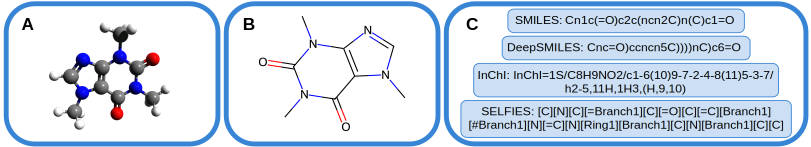
\includegraphics[width=\textwidth]{figures/representations/representations.pdf}
    \caption{Different representations of caffeine. \textbf{A:} 
    Different 1D representations of a molecule. SMILES is an established 
    line notation for molecules. DeepSmiles enables easier generation of
    molecules by getting rid of pair brackets and ring numbers. SELFIES
    guaruantess that a sequence of tokens parses into a valid molecule.
    \textbf{B:} 2D graph representation of a molecule. The nodes represent
    atoms and the edges represent bonds. 
    \textbf{C:} 3D structure of a molecule. The atoms are positioned in 3D
    space. The positions of these atoms can change as some bonds are 
    allow rotations. Source of the 3D structure: \citep{EnglishCaffeine3D2010}.
    \label{fig:molecular-graph}}
\end{figure}
Molecules are complex objects that can be represented in a variety of ways.
While molecules are complex quantum mechanical objects, there exist 
a variety of more simple, practically useful representations of molecules.
Molecules are formed by atoms, which are connected by chemical bonds.
The connectivity between the atoms can be represented as a graph, where
the nodes represent atoms and the edges represent bonds. Additionally,
the atoms/bonds by their atom/bond type and other properties such as
charge or chirality. This representation is called a molecular graph.

Molecules can also be represented as a 3D structure, where the atoms are
positioned in 3D space. This representation is useful for studying the
interactions of molecules with other molecules or proteins. 

Molecular graphs can also be linearized into a 1D sequence of characters. Line
notations such as INCHI \citep{todo} or Simplified Molecular Input Line Entry
System (SMILES) \citep{weiningerSMILESChemicalLanguage1988} represent molecules
as 1D representations of characters. SMILES strings have turned out to be a
highly useful representation of molecules in the context of generative models,
as they are easily processed by sequence-based models such as recurrent neural
networks (RNNs) or transformers \citep{vaswaniAttentionAllYou2017}. Several
extensions for this molecular representation have been proposed, such as SELFIES
\citep{krennSELFIESFutureMolecular2022}, DeepSmiles
\citep{oboyleDeepSMILESAdaptationSMILES2018} or SAFE
\citep{noutahiGottaBeSAFE2023}. 

\subsubsection{Generative models}
There is a wide variety of generative models for molecules, which are based 
on starkly different approaches. 

\paragraph{Autoregressive models} constitute one of the most popular approaches
to generative models for generating discrete 1D/2D molecular representations. 
These models start with an "empty" molecule and iteratively add to it. 
At each step, the model takes the current state of the molecule chooses 
a modification to apply from a set of possible modifications. This modification
is then applied to the molecule and the process is repeated until a special
end-of-sequence action is taken. Mathematically this can be formulated as
\begin{align}
    p(x) = \prod_{i=0}^n p(x_i | x_{0:i-1}), 
\end{align}
where $x$ is the molecule and $x_i$ corresponds to the state of the molecule 
at step $i$. This gives us a probability distribution over the space of molecules
and to evaluate the likelihood of a given molecule. Models for which this fact 
holds are called explicit density models.

One of the most popular approaches is to use recurrent neural networks (RNNs)
or Transformer models \citep{vaswaniAttentionAllYou2017} model 1D sequences.
These models have been used to generate SMILES, SELFIES or DeepSmiles strings
\citep{seglerGeneratingFocusedMolecule2018,todo}. 
In most cases, the training data is a set of molecules and the model is trained
to maximize the likelihood of the training data. The molecules are usually
tokenized into the grammatical units of the used representation before training. 
The model is then trained to predict the next token in the sequence given the
previous tokens.

Another approach to autoregressive modelling is to use graph-based models, which
model the molecular graph directly. These models are based on graph neural
networks (GNNs) and are used to generate molecular graphs directly. 
These models start with an empty graph and iteratively add nodes and edges to
it. At each step the model chooses a modification to apply to the graph and
applies it. While the specification of possible actions is usually more 
complex than in the 1D case, the model can be trained in a similar manner.

\paragraph{Variational autoencoders (VAEs)} are another popular approach to
generate molecules. VAEs are latent space models, which sample 
data by first sampling from a simple latent distribution $p(z)$, which is often 
a multi-variate normal distribution. The samples are then mapped to 
molecular space via a probabilistic decoder network $p(x|z)$.
To make training tractable a second network, the encoder network $q(z|x)$ is
used to map the data to the latent space. The model is trained to maximize
the evidence lower bound (ELBO) of the data
\begin{align}
    \log p(x) \geq \mathbb{E}_{q(z|x)}[\log p(x|z)] - \text{KL}(q(z|x) || p(z)), 
\end{align}
where KL is the Kullback-Leibler divergence. 
This model has the advantage of providing a continuous latent space, which can
be used to interpolate between molecules or run optimization algorithms in
latent space. Calculating the likelihood of a given molecule is not possible
in this model as it requires the integration over the latent space
\begin{align}
    p(x) = \int p(x|z) p(z) dz,
\end{align}
which is usually intractable. This type of model is called an approximate density model. 

\paragraph{Generative adversarial networks (GANs)} are similar to VAEs in that
they also sample from a simple distribution in latent space, $p(z)$ and map the samples to 
molecular space via a generator network $p(x|z)$.
However, the training of GANs is based on a game-theoretic approach, where a
generator network is trained to generate samples that are indistinguishable from
the training data. The training signal is provided by a discriminator network,
which is trained to distinguish between real and generated samples. The generator
is then trained to minimize the discriminator's ability to distinguish between
real and generated samples. GANs have been used to generate molecules 
in a variety of representations \citep{todo}. In general the generator network
is not invertible, which means that the likelihood of a given molecule cannot
be calculated. This makes GANs implicit density models, which define a 
likelihood function $p(x)$ only implicitly via sampling, but not explicitly.


\begin{itemize}
    \item \textbf{Autoregressive models:} Autoregressive models are based on
    recurrent neural networks (RNNs) or transformers \citep{vaswaniAttentionAllYou2017}
    and generate molecules by sampling one atom at a time. 
    \item \textbf{Generative adversarial networks (GANs):} GANs are based on a
    game-theoretic approach, where a generator network is trained to generate
    molecules that are indistinguishable from the training data, while a
    discriminator network is trained to distinguish between real and generated
    molecules.
    \item \textbf{Variational autoencoders (VAEs):} VAEs are based on the idea
    of learning a latent representation of the molecules, which can then be used
    to generate new molecules. 
    \item \textbf{Flow-based models:} Flow-based models are based on the idea of
    learning a bijective mapping between the data space and a latent space. This
    allows for efficient sampling of new molecules.
    \item \textbf{Graph-based models:} Graph-based models are based on the idea
    \item \textbf{3D models:} 3D models are based on the idea of generating 3D
    structures of molecules.
    \item{\textbf{Rule-based methods}} Rule-based methods are based on the idea
    of using a set of rules to generate new molecules. These rules can for example
    be based on chemical reactions or on combining fragments of molecules.
\end{itemize}
    


Triggered by advances in deep learning, the field of generative models for
molecules has seen a surge in interest in recent years. The first deep-learning
based generative models for molecules were based on recurrent neural networks
(RNNs) originally proposed for text generation. After this early work by
\citep{seglerGeneratingFocusedMolecule2018} and
\citep{gomez-bombarelliAutomaticChemicalDesign2018} a great number of different
models have been published
\citep{eltonDeepLearningMolecular2019,sanchez-lengelingInverseMolecularDesign2018}.
These models are based on a large variety of architectures and training
strategies, including autoregressive models, generative adversarial networks
(GANs), variational autoencoders (VAEs), flow-based models
\citep{madhawaGraphNVPInvertibleFlow2019}. One key design choice is the
representation of the molecules, which can be based on SMILES strings,
graph-based representations or 3D structures
\citep{eltonDeepLearningMolecular2019,sanchez-lengelingInverseMolecularDesign2018,pangDeepGenerativeModels2024}.

\subsection{Distribution-learning}
Generative models are often divided into two categories: \emph{goal-directed}
and \emph{distribution-learning} models. Distribution-learning models learn
general structural patterns in molecules and aim to sample novel molecules that
resemble the training data in distribution. These models are then most often
used as a base for goal-directed models, which aim to find molecules that
satisfy a property profile of interest. These properties are usually encoded in
a scoring function, which is then used to guide the generation process, in a
reinforcement learning style feedback loop.

% The evaluation of generative models is challenging. 
While generative models have shown great promise in generating stable chemical
structures their evaluation is often challenging. While evaluation in
discriminative tasks is usually a straightforward evaluation on a hold-out test
set, the evaluation of generative models requires more complex evaluation
schemes and require to take into account various aspects of the generated
molecules. This has led to the development of a range of evaluation metrics
\citep{preuerFrechetChemNetDistance2018,gaoSynthesizabilityMoleculesProposed2020}
and benchmarks for generative models
\citep{polykovskiyMolecularSetsMOSES2020,brownGuacaMolBenchmarkingModels2019}.
However, the evaluation of generative models is still an active area of research
and challenges remain. In this thesis, we address some of these challenges which
are outlined in the following sections.

\subsubsection{Evaluation of distribution-learning models}
The evaluation of distribution-learning methods has posed challenges in
different applications, apart from the generation of molecules. While so called
\emph{likelihood-based} models, such as autoregressive models or flow-based
models, can be evaluated using metrics like the negative log-likelihood or
perplexity evaluated on a hold-out test set, other models such as generative
adversarial networks (GANs) \citep{goodfellowGenerativeAdversarialNetworks2014}
do not offer the possibility of this a straightforward evaluation. To this end
alternative metrics have been proposed, spawning its own subfield of research
\citep{heuselGANsTrainedTwo2017}.

In the field of cheminformatics new metrics have been proposed to evaluate the
quality of generated molecules and how well they match the training data in
distribution \citep{preuerFrechetChemNetDistance2018}.
\citet{polykovskiyMolecularSetsMOSES2020} and
\citet{brownGuacaMolBenchmarkingModels2019} introduced the Moses and GuacaMol
benchmarks respectively, which evaluate the quality of generated molecules using
a combination of metrics. Among these are the FCD metric
\citep{preuerFrechetChemNetDistance2018}, the internal diversity
\citep{benhendaChemGANChallengeDrug2017} of the generated molecules, or the
KL-divergence between the distributions of chemico-physical properties of the
generated molecules and the training data.

It is however not clear how informative these metrics actually are and how well
they correlate with the actual usefulness of the tested generative models.

\subsection{Goal-directed generative models\label{sec:eval-gen}}

In goal-directed generation tasks, the generative models are tasked to find
molecules with a desired property profile. This property profile is usually 
encoded in a scoring function, which assigns a scalar score to each molecule. 
The scoring functions used in these tasks are often based on ML models trained on experimental
data. This can lead to problems, as the optimization process can overfit to
biases of these ML models. 

\subsubsection{Scoring functions}
It is a well-known problem in generative modelling that the optimizing the
output of classification/regression models with respect to their inputs can lead
to unsatisfactory results \citep{todo}. In the context of goal-directed molecule
generators we identified two possible failure modes: Firstly, the generative
models can overfit to artifacts of the scoring function, which are not actually
relevant for the properties of interest. Secondly, the generative models may
overfit to the training samples used to train the scoring function, which can
lead to a lack of novelty in the generated molecules.

\subsubsection{Diversity}
The diversity of the generated molecules is an important aspect in the
application of goal-directed generative models. Given that the scoring functions
are usually only an imperfect and incomplete approximation of the desired
properties, finding a diverse set of molecules that score well can increase the
success chancess of downstream stages of the drug discovery project. Given the
expected failure of some of the candidates in later experiments, having a backup
of other candidates with somewhat different structure can be beneficial.

It is unclear how well current generative models perform in generating diverse
high-scoring molecules, which is due to a combination of two main factors. 
Firstly, many commonly used diversity metrics are inadequate for evaluating
diverse optimization approaches. This results in uninformative benchmarks that
do not meaningfully measure the diversity of the generated molecules. Secondly,
a meaningful comparison of goal-directed generators necessitates a standardized
compute budget. This is because the performance of generative models depends strongly 
on the amount of ressources available for training and evaluation.

\subsubsection{Standardized experimental conditions}
% Introduce the importance of having a benchmark 

\subsubsection{Comparison to relevant baselines}

% \subsubsection{Prediction of molecular properties and virtual screening}
% Machine learning has shown great promise in accelerating the drug discovery
% process. In the context of small molecule drug discovery, machine learning
% methods have been used to predict a range of properties of interest, including
% the activity of a molecule against a target, its pharmacokinetic properties, its
% toxicity or its synthetic accessibility. These predictions can be used to
% prioritize which molecules to test next, to avoid wasting resources on
% unpromising compounds.


\subsection{Retrosynthesis Prediction\label{sec:retrosynthesis}}
% TODO: Add figure explaining retrosynthesis
% Retrosynthesis planning is important and ML can help
Drug candidates, whether suggested by generative models or found by other means,
at some point need to be synthesized in for further testing and 
eventually for use in patients. The synthesis of a molecule is usually a complex
process, involving multiple steps of chemical reactions. Computer-aided synthesis 
planning (CASP) can help by finding new synthesis routes for a target molecule.
In some cases, this can lead to more efficient and cheaper synthesis routes, or
even enables the synthesis of previously inaccessible molecules.

% Synthesis planning 
The most popular approach to CASP is retrosynthesis planning. Starting from a
target molecule, the goal is to predict a chain of chemical reactions that can
transform readily available starting materials into the target molecule. This
problem is usually formulated as a graph search problem, where the nodes are
molecules and the edges are chemical reactions. The goal is to find a path from
the target molecule to a set of starting materials, which can be synthesized in
the laboratory. The connectivity of this graph is given by retrosynthesis
prediction models, which given a target product, predict which reactants it can
be made from. Highly accurate retrosynthesis prediction models are necessary for
the success of CASP tools, as otherwise the suggested synthesis routes might not
be feasible in the laboratory.

% A prominent approach to CASP is template-based planning
% Mention transformers and graph-based models
Template-based models are a popular approach to retrosynthesis prediction. These
models use so called reaction templates, which are graph transformation rules 
that encode connectivity changes between atoms during a chemical reaction. These 
templates can be either automatically extracted from a reaction database or
hand-coded by a chemist. Given a target molecule, the goal is then reframed as a
classification task, where the model predicts which templates can be used to
synthesize the target. Application of the graph transformation rules then leads
to reactants that can be used to synthesize the target molecule. While popular, 
these models have some limitations, in common datasets many templates only occur 
in few training samples, which makes it difficult to train a model that generalizes
well for these rare templates.

In \citep{seidlImprovingFewZeroShot2022} we study the problem of single-step
retrosynthesis prediction. Given a target molecule, the goal is to predict a
set of reactants that can be used to synthesize the target molecule.
Template-based models are a popular approach to single-step retrosynthesis
prediction. These models use so called reaction templates, which are
either extracted from a reaction database or hand-coded by a chemist.
Given a target molecule, the goal is then reframed as a classification task,
where the model predicts which templates can be used to synthesize the target.



\section{Aims and Objectives\label{sec:aims-objectives}}
\subsection{Highlighting Failure Modes in Evaluating Generative Models}
In \citep{renzFailureModesMolecule2019} (\cref{sec:failure-modes}) we show the
limitations of the GuacaMol distribution-learning benchmark, by evaluating the
performance of different sophisticated generative models on this benchmark, and
comparing it to a simple baseline model that generates molecules by introducing
minor variations of the molecules in the training data. We show that the 
most of the tested generative models do not outperform the simple baseline
model, or only do so marginally. This suggests that the tested benchmarks
are not be able to distinguish state-of-the-art generative models 
from simple baseline models, and call for a more comprehensive evaluation of
distribution-learning models. \Cref{sec:failure-modes} reprints
the corresponding publication.

In \citep{renzFailureModesMolecule2019} we introduce \emph{control scores} that
give information whether the optimization overfits to artifacts of the scoring
functions, or the training data. We do this by training additional scoring
functions, trained with either a different random initialization or trained on a
hold-out subset of the the available training data. Using this approach, we can
show that generative models overfit to the scoring function's random
initialization and to high-scoring training samples. This shows that the reported
performance of these models is an overestimation, and that our control 
scores can be used to obtain a more meaningful evaluation of goal-directed 
molecule generators. \Cref{sec:failure-modes} reprints
the corresponding publication.

\subsection{Diversity-based benchmark of goal-directed generators\label{sec:divopt}}
In \citep{renzBenchmarkingEfficiencyGenerative2024} we introduce a benchmark for
diverse optimization that addresses the above-mentioned issues. In this
benchmark, we evaluate the diversity of the generated molecules using a recently
proposed diversity metric \#Circles \citep{xieHowMuchSpace2023}. We compare the
performance of diverse optimization approaches under two different compute
budgets, namely a fixed number of scoring function evaluations and a fixed time
budget. The first setting is relevant for applications where the cost of
evaluating the scoring function dominates the optimization process, while the
second setting is relevant for scoring functions that are cheap to evaluate.
Using this setup we test 14 goal-directed optimization methods and show how
SMILES-based auto-regressive models dominate the benchmark.
\Cref{sec:diverse-efficiency} reprints the corresponding publication.

\subsection{Improving few-shot and zero-shot retrosynthesis prediction}
In \citep{seidlImprovingFewZeroShot2022} we propose a novel approach to
template-based retrosynthesis prediction. We use a multimodal learning approach
that learns to associate relevant templates to product molecules using a Modern
Hopfield Network \citep{ramsauerHopfieldNetworksAll2020}. Our model can leverage
structural information about the templates and can make use of similarities
between them. This allows for improved generalization, especially for templates
with few training samples and even for unseen templates. This model is several
times faster than comparable methods and shows good predictive performance.
\Cref{sec:mhn-react} reprints the corresponding publication.

\section{List of publications\label{sec:publications}}
This thesis comprises the work published in the following papers:

\begin{itemize}
    \item \fullcite{renzFailureModesMolecule2019}
    \item \fullcite{renzBenchmarkingEfficiencyGenerative2024}
    \item \fullcite{seidlImprovingFewZeroShot2022}
\end{itemize}



% give overview over my other publications
\paragraph{Other Publications} Besides the papers listed above, I have also
contributed to the following publications:

\begin{itemize}
    \item \fullcite{preuerFrechetChemNetDistance2018}
    \item \fullcite{renzUncertaintyEstimationMethods2019}
    \item \fullcite{hofmarcherLargescaleLigandbasedVirtual2020}
    \item \fullcite{renzLowCountTimeSeries2023}
\end{itemize}